\documentclass[sigconf]{acmart}

\usepackage{booktabs} % For formal tables
\usepackage{bm} % For formal tables


% Copyright
%\setcopyright{none}
%\setcopyright{acmcopyright}
%\setcopyright{acmlicensed}
\setcopyright{rightsretained}
%\setcopyright{usgov}
%\setcopyright{usgovmixed}
%\setcopyright{cagov}
%\setcopyright{cagovmixed}


%\let\jnl@style=\rmfamily 
%\def\ref@jnl#1{{\jnl@style#1}}% 
\newcommand\rsquo{'}
          % Astronomical Journal 
\newcommand\aj{{AJ}}% 
          % Astronomical Journal 
\newcommand\araa{{ARA\&A}}% 
          % Annual Review of Astron and Astrophys 
\newcommand\apj{{ApJ}}% 
          % Astrophysical Journal 
\newcommand\apjl{{ApJ}}% 
          % Astrophysical Journal, Letters 
\newcommand\apjs{{ApJS}}% 
          % Astrophysical Journal, Supplement 
\newcommand\ao{{Appl.~Opt.}}% 
          % Applied Optics 
\newcommand\apss{{Ap\&SS}}% 
          % Astrophysics and Space Science 
\newcommand\aap{{A\&A}}% 
          % Astronomy and Astrophysics 
\newcommand\aapr{{A\&A~Rev.}}% 
          % Astronomy and Astrophysics Reviews 
\newcommand\aaps{{A\&AS}}% 
          % Astronomy and Astrophysics, Supplement 
\newcommand\azh{{AZh}}% 
          % Astronomicheskii Zhurnal 
\newcommand\baas{{BAAS}}% 
          % Bulletin of the AAS 
\newcommand\jrasc{{JRASC}}% 
          % Journal of the RAS of Canada 
\newcommand\memras{{MmRAS}}% 
          % Memoirs of the RAS 
\newcommand\mnras{{MNRAS}}% 
          % Monthly Notices of the RAS 
\newcommand\pra{{Phys.~Rev.~A}}% 
          % Physical Review A: General Physics 
\newcommand\prb{{Phys.~Rev.~B}}% 
          % Physical Review B: Solid State 
\newcommand\prc{{Phys.~Rev.~C}}% 
          % Physical Review C 
\newcommand\prd{{Phys.~Rev.~D}}% 
          % Physical Review D 
\newcommand\pre{{Phys.~Rev.~E}}% 
          % Physical Review E 
\newcommand\prl{{Phys.~Rev.~Lett.}}% 
          % Physical Review Letters 
\newcommand\pasp{{PASP}}% 
          % Publications of the ASP 
\newcommand\pasj{{PASJ}}% 
          % Publications of the ASJ 
\newcommand\qjras{{QJRAS}}% 
          % Quarterly Journal of the RAS 
\newcommand\skytel{{S\&T}}% 
          % Sky and Telescope 
\newcommand\solphys{{Sol.~Phys.}}% 
          % Solar Physics 
\newcommand\sovast{{Soviet~Ast.}}% 
          % Soviet Astronomy 
\newcommand\ssr{{Space~Sci.~Rev.}}% 
          % Space Science Reviews 
\newcommand\zap{{ZAp}}% 
          % Zeitschrift fuer Astrophysik 
\newcommand\nat{{Nature}}% 
          % Nature 
\newcommand\iaucirc{{IAU~Circ.}}% 
          % IAU Cirulars 
\newcommand\aplett{{Astrophys.~Lett.}}% 
          % Astrophysics Letters 
\newcommand\apspr{{Astrophys.~Space~Phys.~Res.}}% 
          % Astrophysics Space Physics Research 
\newcommand\bain{{Bull.~Astron.~Inst.~Netherlands}}% 
          % Bulletin Astronomical Institute of the Netherlands 
\newcommand\fcp{{Fund.~Cosmic~Phys.}}% 
          % Fundamental Cosmic Physics 
\newcommand\gca{{Geochim.~Cosmochim.~Acta}}% 
          % Geochimica Cosmochimica Acta 
\newcommand\grl{{Geophys.~Res.~Lett.}}% 
          % Geophysics Research Letters 
\newcommand\jcp{{J.~Chem.~Phys.}}% 
          % Journal of Chemical Physics 
\newcommand\jgr{{J.~Geophys.~Res.}}% 
          % Journal of Geophysics Research 
\newcommand\jqsrt{{J.~Quant.~Spec.~Radiat.~Transf.}}% 
          % Journal of Quantitiative Spectroscopy and Radiative Trasfer 
\newcommand\memsai{{Mem.~Soc.~Astron.~Italiana}}% 
          % Mem. Societa Astronomica Italiana 
\newcommand\nphysa{{Nucl.~Phys.~A}}% 
          % Nuclear Physics A 
\newcommand\physrep{{Phys.~Rep.}}% 
          % Physics Reports 
\newcommand\physscr{{Phys.~Scr}}% 
          % Physica Scripta 
\newcommand\planss{{Planet.~Space~Sci.}}% 
          % Planetary Space Science 
\newcommand\procspie{{Proc.~SPIE}}% 
          % Proceedings of the SPIE 
\let\astap=\aap 
\let\apjlett=\apjl 
\let\apjsupp=\apjs 
\let\applopt=\ao 

% DOI
\acmDOI{10.475/123_4}

% ISBN
\acmISBN{123-4567-24-567/08/06}

%Conference
\acmConference[SC17]{SC17}{November 2017}{Denver,
  Co, USA} 
\acmYear{2017}
\copyrightyear{2017}

\acmPrice{15.00}


\begin{document}
\title{Extreme-scale global simulation of planetary rings on TaihuLight}
\titlenote{Produces the permission block, and
  copyright information}
\subtitle{Extended Abstract}
\subtitlenote{The full version of the author's guide is available as
  \texttt{acmart.pdf} document}


\author{Masaki Iwasawa}
%\orcid{1234-5678-9012}
\affiliation{%
  \institution{RIKEN AICS}
  \streetaddress{7-1-26 Minatojima-minami-machi}
  \city{Chuo-ku, Kobe} 
  \state{Hyogo}
  \postcode{ 650-0047}
  \country{Japan}
}
\email{masaki.iwasawa@riken.jp}

\author{Long Wang}
%\orcid{1234-5678-9012}
\affiliation{%
  \institution{RIKEN AICS}
  \streetaddress{7-1-26 Minatojima-minami-machi}
  \city{Chuo-ku, Kobe} 
  \state{Hyogo} 
  \postcode{ 650-0047}
  \country{Japan}
}
\email{long.wang@riken.jp}

\author{Keigo Nitadori}
%\orcid{1234-5678-9012}
\affiliation{%
  \institution{RIKEN AICS}
  \streetaddress{7-1-26 Minatojima-minami-machi}
  \city{Chuo-ku, Kobe} 
  \state{Hyogo} 
  \postcode{ 650-0047}
  \country{Japan}
}
\email{keigo@riken.jp}

\author{Daisuke Namekata}
%\orcid{1234-5678-9012}
\affiliation{%
  \institution{RIKEN AICS}
  \streetaddress{7-1-26 Minatojima-minami-machi}
  \city{Chuo-ku, Kobe} 
  \state{Hyogo} 
  \postcode{ 650-0047}
  \country{Japan}
}
\email{daisuke.namekata@riken.jp}

\author{Miyuki Tsubouchi}
%\orcid{1234-5678-9012}
\affiliation{%
  \institution{RIKEN AICS}
  \streetaddress{7-1-26 Minatojima-minami-machi}
  \city{Chuo-ku, Kobe} 
  \state{Hyogo} 
  \postcode{ 650-0047}
  \country{Japan}
}
\email{miyuki.tsubouchi@riken.jp}



\author{Jun Makino}
%\orcid{1234-5678-9012}
\affiliation{%
  \institution{RIKEN AICS}
  \streetaddress{7-1-26 Minatojima-minami-machi}
  \city{Chuo-ku, Kobe} 
  \state{Hyogo} 
  \postcode{ 650-0047}
}
\email{jmakino@riken.jp}


\author{Zhao Liu}
%\orcid{1234-5678-9012}
\affiliation{%
  \institution{National Supercomputing Center in Wuxi}
%  \streetaddress{7-1-26 Minatojima-minami-machi}
  \city{Wuxi} 
%  \state{Hyogo} 
%  \postcode{ 650-0047}
  \country{China}
}
\email{liuzhao@mail.nsccwx.cn}


\author{Haohuan Fu}
%\orcid{1234-5678-9012}
\affiliation{%
  \institution{Department of Earth System Science, Tsinghua University}
  \city{Beijing} 
  \country{China}
}
\email{haohuan@tsinghua.edu.cn}

\author{Guangwen Yang}
%\orcid{1234-5678-9012}
\affiliation{%
  \institution{Department of Computer Science and Technology, Tsinghua University}
  \city{Beijing} 
  \country{China}
}
\email{ygw@tsinghua.edu.cn}





% The default list of authors is too long for headers}
\renewcommand{\shortauthors}{M. Iwasawa et al.}


\begin{abstract}
In this paper, we report the measured performance of TaihuLight system
for extreme-scale, global simulation of planetary rings with up to 1
trillion particles. Global simulation of ring systems have become
possible only recently, and typical number of particles used is still
much less than 1 billion. We have ported our framework for
particle-based simulation, FDPS, to TaihuLight system successfully, to
use it for extreme-scale simulations necessary to study interactions
between satellites and rings and structures induced by satellites.
FDPS uses Barnes-Hut tree algorithm and domain decomposition with
automatic load-balancing. The measured performance is around 11\% of
the theoretical peak, while the efficiency of the
interaction kernel is currently around 50\%.
general considerations on performance optimization on heterogeneous
systems such as TaihuLight.
\end{abstract}

%
% The code below should be generated by the tool at
% http://dl.acm.org/ccs.cfm
% Please copy and paste the code instead of the example below. 
%
 \begin{CCSXML}
<ccs2012>
<concept>
<concept_id>10010405.10010432.10010435</concept_id>
<concept_desc>Applied computing~Astronomy</concept_desc>
<concept_significance>500</concept_significance>
</concept>
</ccs2012>
\end{CCSXML}

 \ccsdesc[500]{Applied computing~Astronomy}
%%  \begin{CCSXML}
%% <ccs2012>
%%  <concept>
%%   <concept_id>10010520.10010553.10010562</concept_id>
%%   <concept_desc>Computer systems organization~Embedded systems</concept_desc>
%%   <concept_significance>500</concept_significance>
%%  </concept>
%%  <concept>
%%   <concept_id>10010520.10010575.10010755</concept_id>
%%   <concept_desc>Computer systems organization~Redundancy</concept_desc>
%%   <concept_significance>300</concept_significance>
%%  </concept>
%%  <concept>
%%   <concept_id>10010520.10010553.10010554</concept_id>
%%   <concept_desc>Computer systems organization~Robotics</concept_desc>
%%   <concept_significance>100</concept_significance>
%%  </concept>
%%  <concept>
%%   <concept_id>10003033.10003083.10003095</concept_id>
%%   <concept_desc>Networks~Network reliability</concept_desc>
%%   <concept_significance>100</concept_significance>
%%  </concept>
%% </ccs2012>  
%% \end{CCSXML}

%% \ccsdesc[500]{Computer systems organization~Embedded systems}
%% \ccsdesc[300]{Computer systems organization~Redundancy}
%% \ccsdesc{Computer systems organization~Robotics}
%% \ccsdesc[100]{Networks~Network reliability}

% We no longer use \terms command
%\terms{Theory}

\keywords{ACM proceedings, \LaTeX, text tagging}


\maketitle

\section{Justification for ACM Gordon Bell Prize}

% 50 wiords max

We have achieved 11\% of the theoretical peak performance, or 10.1
Pflops, on the Sunway TaihuLight system, for the global simulation of
planetary rings including shepherding satellites. The algorithm used
is the Barnes-Hut tree. We have incorporated many new
techniques to achieve high efficiency on the heterogeneous Sunway
processor.

\section{Performance Attributes}

  \begin{tabular}{ll}
    \toprule
    Category of achievement&  scalability, time-to-solution,\\
                           &peak performance\\
    Type of method used & Explicit with\\
                        &long-range interaction\\    
    Results reported on the basis of&  whole application\\
                                   &including I/O\\
     Precision reported &  double precision\\
     System scale & results measured on \\
                  &full-scale system\\
    Measurement mechanism &   FLOP count\\

  \bottomrule
\end{tabular}

  \section{Overview of the Problem}
  \label{sect:overview}

%    description of the problem and its importance, in terms
%    understandable to a non-specialist (1 p max)

Saturn's ring was found by Galileo Galilei in 1610. For more than
three centuries, it had been the only known ring system within our
solar system. In 1977, Rings of Uranus were found through ground-based
observations, and then in 1979 Rings of Jupiter by Voyager 1 and in
1989 those of Neptune by Voyager 2.  Very recently, it turned out that
some of minor planets also have rings. The first distinctive example
is 10199 Chariklo, whose orbit is between those of Saturn and Uranus
(and thus one of Centaurs). There are probably  more Centaurs with rings.

In 2015, it was announced that a very large and complex ring system is
found around an planet of a star ``1SWASP J140747.93-394542.6''. In 
April and May 2007, the star showed quite complex change of
brightness, which was interpreted  as the result of eclipses of the
star by the planetary rings. If this interpretation is correct, the
ring is huge, with the outer radius of 90 million km (0.6 AU). For
comparison, Saturn's F Ring has the radius of $1.4\times 10^5{\rm
  km}$, and even the outer radius of the very faint E ring is less
than $5\times 10^5{\rm km}$. 
Thus, quite recently, a wide variety of ring systems have been found.
How these rings are formed and have evolved is an important question
in planetary science.

Our understanding of the structure of the rings have been advanced
greatly, mainly through interplanetary missions such as Voyager 1 and
2, and most recently Cassini. Through these missions, a number of new
findings have been made. Among the new findings, probably the most
surprising is that the rings show dynamic changes of structures,
possibly including the formation of new satellites. Another example of
truly new findings of the Cassini mission is the vertical structure at
the outer edge of the B ring.  Other new findings include axisymmetric
structures of a vast range of scales, from 100m to 100km.

For some of these new findings, theoretical explanation based on fluid
approximation has been made. However, many of them cannot be explained
with simple fluid models, and more realistic treatment of ring as
collection of particles interacting through both mutual gravity and
physical collisions is necessary. 

Planetary rings are usually at the radii around the Roche limit. Thus,
mutual gravity between particles does not easily  lead to the
formation of new satellites, but is important enough to form spiral
waves (``wakes'') in very small scales, which increases the effective
viscosity and should enhance the radial transport of the angular
momentum. On the other hand, the actual ring system seems to consist of very
large number of very narrow rings, separated with distinct gaps. It is
believed that high-order resonances with small embedded satellites
(so-called moonlets), but whether or not such gaps can be formed by
resonances has not been fully understood. 

Very little simulation-based studies have been done to understand
these new findings. The primary reason for this lack is simply that
simulations of such structures must be global simulations including
self gravity of ring particles, which would require very large number
of particles and thus very large amount of  computing resources.

Up to now, most of simulations of ring structures have been local
ones, in which a small patch  was cut out from the ring and simulated
under the assumption of the local Hill approximation and periodic
boundary condition \cite{WisdomTremaine1988}. Rein and Latter
\cite{ReinLatter2013} performed ``Large-scale'' simulation of viscous
overstability in Saturn's rings, using up to 204,178 particles and up
to 10,000 orbits using this local approach.  Because very long
simulations are necessary, the number of particles has been
small. They used {\tt REBOUND} \cite{ReinLiu2012}, an MPI-parallel
$N$-body simulation code.



We should note that even though the simulations so far done in this
field is relatively small, that does not mean there is no need or
possibilities for larger scale simulations. If we want to study the
global structures of rings, we cannot rely on local treatment. For
example, the effect of resonances with small satellites can only be
studied using global simulations. On the other hand, the number of
particles one need for global simulations, even  for a very narrow
radial range, is very large. For example, consider A ring of Saturn
with the radius of around $1.3\times 10^5\rm km$. The typical radius
of ring particles is 6 m\cite{ZEBKER1985531}, and the optical depth of
the ring is around unity. Thus, we need $10^4$ particles per $\rm
km^2$ or around $10^{12}$ particles for the radial range of 100
km. With this radial range, we can model many of fine features observed
by Cassini directly.

Compared to the size of local simulations performed so far, the number
of particles necessary for global simulations might seem too
large. However, such large simulations are not beyond the reach of
present-day supercomputers. 

We have developed a framework for developing fast and highly scalable
codes for particle-based simulations,
FDPS\cite{Iwasawaetal2016}. Using FDPS, Michikoshi and Kokubo
\cite{MichikoshiKokubo2017} performed global simulations of rings with
probably the largest number of particles. They used 300M particles to
model two narrow rings of Chariklo. Thus the number of particles they
used is already three orders of magnitude larger than what have been
used for global simulations. They have used Cray XC30 at the Center of
Computational Astrophysics, National Astronomical Observatory of
Japan, with the peak speed of 1 Pflops.  In order to model fine
structures of Saturn's rings, we need to increase the number of
particles by another three orders of magnitude. Such an increase is
now within reach of big machines with the peak speef in the range of
100PF, such as the Sunway TaihuLight system with the peak speed of
125PF.


\section{Current State of the Art}


%   quantitative discussion of current SoA, with emphasis on
%   performance-related aspects  (1 p max)   

% GreeM 1.800e10 particle steps/sec


Simulation study of planetary rings has a long history. Almost all
simulations have been performed using the local approximation,
following the treatment first proposed by Wisdom and
Tremaine\cite{WisdomTremaine1988}. {\tt REBOUND}\cite{ReinLiu2012} 
is an open-source code designed for such local simulations and have
been used in a number of recent studies. Since {\tt REBOUND} is
designed for local simulation of planetary rings, it adopts a simple
regular, equal-sized  grid for domain decomposition. Its measured
performance is $\sim 8,000$ particle steps per second per MPI process,
on a cluster of AMD quad-core Barcelona processors (clock speed not
reported in the paper). The force calculation algorithm is Barnes-Hut
tree\cite{BarnesHut1986} with the opening angle $\theta=0.7$. The
calculation cost is not discussed in detail in their paper, but with
BH tree for nearly two-dimensional system, the average number of
interactions per particle would be around 500 for $\theta=0.7$. Thus,
REBOUND handles around $4\times 10^6$ particle-particle interactions
per second per core, on an AMD Barcelona processor with the peak speed
of around 10 Gflops (double precision). 

Rein and Latter \cite{ReinLatter2013}  used {\tt REBOUND} to simulate
up to 200k particles for up to 10,000 orbits. More recently,
Ballouz {\it et al.}\cite{Ballouzetal2017} used {\tt
  pkdgrav}\cite{Stadel2001}  for simulations with up to 500k
particles.

Michikoshi and Kokubo \cite{MichikoshiKokubo2017} performed global
simulations of rings with 300M particles, using
FDPS\cite{Iwasawaetal2016}. They so far followed the system only for
10 orbital periods.

The total calculation cost is roughly proportional to number of
particles multiplied by the number of orbital periods followed, since
the calculation cost per timestep is $O(N \log N)$ when Barnes and Hut
tree algorithm is used and the number of timestep required for ring
simulations is essentially independent of the number of
particles. Thus, we can conclude that the size of state-of-the-art
simulations of planetary rings is around $10^9$ particle-orbits, or
around $10^{12}$ particle-steps.

We should note that even though the simulations so far done in this
field is relatively small, that does not mean there is no need or
possibilities for larger scale simulations. If we want to model the
global structures of rings, we cannot rely on local treatment. For
example, the effect of resonances with small satellites can only be
studied using global simulations. On the other hand, the number of
particles one need for global simulations, even  for a very narrow
radial range, is very large. For example, consider A ring of Saturn
with the radius of around $1.3\times 10^5\rm km$. The typical radius
of ring particles is 6 m\cite{ZEBKER1985531}, and the optical depth of
the ring is around unity. Thus, we need $10^4$ particles per $\rm
km^2$ or around $10^{12}$ particles for the radial range of 100
km. With this radial range, we can model many of fine features observed
by Cassini directly.

If we could use particles with larger size, we could reduce the number
of particles required significantly. However, that would change the
viscous diffusion timescale of the ring, and thus  what would be observed. Thus, if at all possible, it is
desirable to perform simulations with particle of real physical
radius, which  would require at least $10^{16}$ and ideally $10^{19}$ particle
steps.

In other fields of astrophysics, very large simulations have been
performed. For example, Ishiyama\cite{Ishiyama2014} used $4096^3$
particles to follow the formation and growth of dark matter halos of
smallest scales. This simulation corresponds to  $10^{16}$ particle
steps. Part of this calculation was performed on K computer. The
performance of K computer is $4.0\times 10^{10}$ particle steps per
second on the entire K computer, or 60,000 particle step per second
per core for a processor core with the theoretical peak performance of
16 Gflops\cite{Ishiyamaetal2012}. The efficiency they achieved is 55\%
of the theoretical peak. 

The simulation algorithm used is quite similar for dark matter
simulation and simulation of planetary rings, except that we need the
treatment of physical collisions between particles in the latter. This
means that, in addition to the calculation of $1/r$ gravitational
force, we need to add repulsive force and velocity-dependent drag
force, if two particles are physically overlapped. This treatment of
course increases the calculation cost of particle-particle
interaction, but otherwise the simulation algorithm is quite similar.


In large simulations as those reported in \cite{Ishiyamaetal2012},
simulation algorithm used are largely similar. All of them use domain
decomposition and Barnes and Hut tree algorithm. For domain
decomposition, several variations have been used, such as
Orthogonal Recursive Bisection\cite{Salmon1990}, Hashed Oct
Tree\cite{WarrenSalmon1992}, Multisection\cite{Makino2004}.

One difference between cosmological simulations and other simulations
is that in cosmological simulations the periodic boundary conditon is
used. For most of other simulations, open boundary is used. The
calculation cost of particle-particle interaction is usually lower for
periodic boundary, since we can use the TreePM
algorithm\cite{Bagla2002}, in which the long-range $1/r$ potential is
divided into long-range and short-range terms. Long range term is
evaluated using particle-mesh method, and only the short-range part is
evaluated with the tree method. For open boundary we cannot apply such
cutoff, and thus the calculation cost is generally somewhat higher for
open boudary problems than for periodic boundary problems. 


Efficient implementations on large-scale GPGPU clusters
exist\cite{Hamadaetal2009, PortegiesZwartetal2014,Bedorfetal2014}.
B{\'e}dorf {\it et al.} performed the simulation of Milky Way Galaxy
  using $2.42 \times 10^{11}$ particles. The achieved performance is
  24.77 Pflops on ORNL Titan, and one timestep took 5.5 seconds. Thus
  they have achieved the performance of $4.4 \times 10^{10}$ particle
  steps per seconds. The theoretical peak performance of Titan is 73.2
  Pflops in single precision. Thus, the achieved efficiency is 33.8\%.

So far, there is no report on the implementation and performance of
parallel tree algorithm on processors with a heterogeneous
architecture such as Sunway TaihuLight.  In this paper, we present the
result of our effort to implement the parallel tree algoritm on Sunway
TaihuLight. 


\section{Sunway TaihuLight}

In this section, we briefly describe the features of the Sunway
TaihuLight system and its SW26010 processor, related to the
performance and necessary modifications of the algorithm.

The TaihuLight system consists of 40960 nodes, connected by the
network with injection bandwidth of 8GB/s per node. The hardware network
bandwidth is large enough for our purpose.

The processor itself consists of four CGs (core groups), each with one
MPE (management processing element) and 64 CPEs (computing processing
elements). Both MPE and CPE are 64-bit RISC cores. MPE has L1 cache
memories for  both instructions and data, and also L2 data cache. On
the other hand, each CPE has L1 instruction cache and 64KB of local
data memory. CPEs can communicate with the main memory through DMA.
Each CPE can initiate multiple asynchronous DMA operations. Thus, it is
possible to write the kernel loop so that the computation, DMA read
for the data which will be necessary for the next iteration, and DMA
write operation of the result of the previous iteration all run
concurrently and thus the communication with the main memory is
completely hidden. This capability of explicit control of
communication with main memory is crucial for achieving high
efficiency, as will be discussed in section \ref{sect:innovation}.


Each core group is connected to 8GB DDR3 DRAM with the theoretical
peak transfer rate of 34GB/s. The processor runs at the clock
frequency of 1.45GHz, and each core (both MPE and CPE) can perform
four double precision FMA operations. Thus, the theoretical peak
performance of one processor is 3016 Gflops and that of one CG is 754
Gflops.

CPEs in one CG are organized into an $8\times 8$ array, and within
each row or column, low-latency, high-bandwidth point-to-point and
broadcast communications are supported.

Operating system runs on MPE, and by default the user program also
runs on MPE. In order to use CPEs, there are two ways. One is to use an
extension of OpenACC designed for SW26010 processor, and the other is
use a lightweight thread library called Athread. Athread is more
difficult to use compared to OpenACC, but allows fine-grained control
of CPEs. 

Because of its heterogeneous structure, one might imagine that SW26010 is
similar to systems with GPGPUs. However, there are several important
differences between systems with GPGPUs and SW26010. The largest one
which makes the strategy for program development completely different
is the fact that, even though the code on CPE side should use DMA, the
memory bandwidth of CPEs combined is much higher than that of
MPE. This is true not only for continuous access but also for random
access.

In the case of GPGPU, there is the communication  bottleneck between
CPU memory and GPU memory, and thus we need to carefully design the
algorithm so that the communication between CPU and GPU is minimized.
In the case of the SW26010 processor, Using CPEs for main memory
access is actually faster than using MPE. Thus, almost any operation
is actually faster on CPEs than on MPE, at least when implemented
carefully using Athread and asynchronous DMA operations. 

Since the data move between the main memory and CPE is faster than
that between MPE and main memory, the strategy for program
optimization for SW26010 is quite different from that for GPGPU and
actually much closer to that for traditional vector processors. Almost
any loop which is reasonably long can get benefit from moving to CPE.
Of course, since the memory bandwidth of CPEs is very small compared
to their floating-point arithmetic performance, we then need to write
the kernel code so that it does as many calculations as possible.

Thus, as in the case of vector processors, the performance
optimization on SW26010 can be done step-by-step, one-loop-at-a-time
way. This means the debugging is relatively easy and thus development
cycle is actually pretty fast.

One problem of current software on SW26010 is that the optimization
capability of the compiler for CPE is rather limited. Thus, in order
to achieve the efficiency close to the theoretical peak performance
for the inner kernels, it is currently necessary to manually schedule
instructions through writing the innermost kernel in assembly
language. 


\section{Innovations Realized}
  \label{sect:innovation}.
%   what the innovations are and how they were achieved (2 pp max)

% 書くべきこと:

% 従来の方法では、相互作用計算の高速化にほぼ集中していたこれは、ツリー
% 法ではそこが計算時間の95% 以上を占めるからであるしかし、Sunway では、
% MPE の能力(ベクトル化されてないと特に)とCPE の能力には、数百倍の開き
% がある。従って、従来のやり方では十分ではない。可能なアプローチとして
% は、

% 1) MPE で行う必要がある複雑な処理の回数を減らす
%   相互作用リストを記憶し、ツリー構造も記憶する
% 2) 従来汎用プロセッサで行っていた処理も、処理量が多いところから順次
% CPE に移動する

% ここで注意するべきことは、MPE 単体では主記憶のバンド幅を使い切ること
% が容易ではないので、性能が主記憶のバンド幅リミットであるオペレーショ
% ンでも、CPE にやらせるほうが数倍速いことである。もちろん、

% ソートはどうしたんだっけ?

In this section, we  describe our implementation of simulation code
for self-gravitating planetary ring in detail, focusing on the
difference from previous implementations on large-scale parallel
systems with accelerators.

The following gives the usual steps for highly parallel code for
self-gravitating particle system:

\begin{enumerate}

  \item Perform domain decomposition
  \item Exchange particles so that particles belong to appropriate domains
  \item Perform interaction calculation using fast algorithm such as
    Barnes-Hut tree
  \item Integrate the orbits of particles
  \item go back to step 1.

\end{enumerate}

In the case of approaches with local essential tree, step (3) consists
of the following substeps:

\begin{description}

\item{(3a)} Construct the ``local'' tree structure from particles in
  the domain
\item{(3b)} Collect the information necessary for the calculation of
  interaction from other processes (so called local essential tree)
\item{(3c)} Construct the ``global'' tree from the collected information
\item{(3d)} For small groups of particles, traverse the tree and
  calculate the interaction. Repeat this for all groups.
\end{description}
In the original algorithm\cite{BarnesHut1986}, the traversal of the
tree is done for each particle, and force calculation is done during
the traversal. However, on almost all modern implementation, following
the idea of Barnes\cite{Barnes1990}, tree traversal is done for a
group of neighboring particles, which is constructed using the tree
structure itself. During the traversal, list of particles and tree
nodes which exert the force on this group of particles is constructed,
and actual force calculation is done through the double loop over
particles in the group and those in the list. This structure makes it
possible to use vector pipelines, scalar SIMD units, and even
special-purpose computers\cite{Makino1991c} with high efficiency. For
GPGPUs, the extension of this algorithm, in which multiple pairs of
this group and list are constructed and then passed to GPGPU, is
used\cite{Hamadaetal2009}. Even in the case of special-purpose
computers or GPGPUs, in this algorithm, all computations, except for
the actual interaction calculation in the double loop, is done on
general-purpose front-end computer.

In the following we call this
approach the accelerator-minimal approach, since the part of the code
which is executed on the accelerator (or SIMD hardware or
special-purpose computers) is minimized, so that the amount of work of
porting is small.  This approach has been quite successful for many
different platforms. 

Another approach is to port more work to accelerator side. Parallel
algorithms exist for both the tree traversal and tree construction,
and thus it is possible to implement them on GPUs\cite{Bedorfetal2012}. 
Even though the efficiency of the code for tree construction and tree
traversal is not so high as that for interaction calculation, this
approach is potentially better on GPGPU systems than
accelerator-minimal approach, since we can remove the bottleneck of
data transfer and in some cases tree handling on the front-end
computer. We call this approach the accelerator-maximal approach.

Before we started porting FDPS to SW26010, we made a rough estimate on
what performance we can achieve using these two approaches. It turned
out the performance we can achieve with the accelerator-minimal
approach is far from satisfactory, simply because  MPE is too slow. We
estimated that the time for MPE to perform the tree construction and
tree traversal is more than 10 times longer than that for CPEs to do
the interaction calculation, if the efficiency of the interaction
kernel is reasonably high like 30-40\%. Thus, traditional approach for
Barnes-Hut tree algorithm is not sufficient for SW26010. 

The accelerator-maximal approach would be certainly better than 
the accelerator-minimal approach for SW26010, if can be implemented in
a reasonable time. However, even when the accelerator-maximal approach
is adopted, getting reasonable efficiency turned out to be not easy,
since then the performance of tree construction and tree traversal
would be limited by the bandwidth of the main memory for random
access.

Thus, it is necessary to introduce some new approach to reduce the
calculation (or main memory access) cost of operations other than the
interaction calculation.  We adopted the neighbor-list method used
in molecular-dynamics simulations with short-range interactions.

The idea of the neighbor-list method is, roughly speaking, to create
the list of particles with which one particle interact, and use the
same list for multiple timesteps. By doing so, we can reduce the cost
of construction of the neighbor list significantly. Of course, we
need to increase the neighbor list, so that it contain all particles
which might go into the interaction radius of the particle.

Usually, in the case of self-gravitating systems, it is rather
difficult to use such neighbor lists, since particles move relatively
large distance compared to the interparticle distance in one timestep.
However, in the case of the simulation of planetary ring, typical
relative velocity between particles is small and particles move only
very small distance compared to the interparticle distance. This is
because of the physical nature of the system. The ring is physically
very thin, and the optical depth of the ring is around unity. The ring
particles are moving in nearly circular orbits. However, since the
average interparticle distance in the ring plane is of the order of
the particle radius itself, there are frequent physical
collisions. Since the physical collisions are inelastic, they reduce
the random relative velocities of ring particles.

Thus, unlike in the case of dark matter halo simulation or galactic
dynamics simulations, in planetary ring simulations, relative
velocities of neighboring particles is very small, and particles move
only a small fraction of the interparticle distance in one
timestep. Thus, we can use the interaction list constructed for the
interaction calculation, typically for several tens of timestep,
without increasing the length of the interaction list significantly. 

By using this persistent interaction list, we can reduce the
calculation cost of the part other than the interaction calculation
drastically. While we are using the same interaction list, we skip the
domain decomposition, exchange of particles, construction of the local
tree. We still need to update the physical quantities of the nodes of
the local tree, since particles in the lowest level have moved. Then,
using the list of nodes for the local essential tree, the
communication between the nodes is performed. Finally, the physical
quantities of the global tree is updated, and the force calculation is
performed using this updated global tree and the persistent
interaction list.

When we use the (persistent) interaction list, what we usually do is
first create the contiguous array of physical quantities of particles,
by scanning the interaction list (of either pointers or indices of
particles) and copy the physical quantities from original particle
data to arrays. In our current implementation, we actually avoid this
copy, and load (using DMA) particles during the interaction
calculation. Since this DMA operation is done concurrently with the
actual calculation itself, it is completely hidden, and relatively low
performance due to small DMA size does not hurt the total
performance. 

We have ported all operations in timesteps in which the interaction list
is used (list-using step), except for MPI functions for communication, to CPEs. For the
timestep in which the interaction list is constructed (list-constructing
step), some operations are still  done on MPE. These include the tree
traversal and determination of the distination process of particles
which moved out of the domain of the process.



%% \begin{table}
%%   \caption{Calculation times for original and new approach}
%%   \label{tab:improvement}
%%   \begin{tabular}{lccc}
%%     \toprule
%%     Operation & Original & New & speedup\\
%%     \midrule
%%     Tree construction & & &\\
%%     Local moment & & &\\
%%     LET construction & & &\\
%%     LET communicaton & & &\\
%%     Global  moment & & &\\
%%     Interaction List construction & & &\\
%%     Interaction calculation & & &\\
%%     \midrule
%%     Total & & &\\
%%   \bottomrule
%% \end{tabular}
%% \end{table}

%% Table \ref{tab:improvement} shows the speedup factor we achieve over
%% the original accelerator-minimal approach, for the case of using the
%% interaction list for 64 timesteps. 


\begin{table}
 \caption{Initial condition for weak scaling runs}
 \label{tab:initialcoditions}
 \begin{tabular}{lc}
   \toprule
   Central planet & Saturn\\
   Ring inner radius & $10^5$ km\\
   Ring width        & $10^4$ km\\
   Number of MPI processes & 32768 -- 131072 \\
   Number of particles per process & $3.4 \times 10^{10} $ -- $1.4 \times 10^{11}$  \\
   particle radius & 60 -- 120 m\\
 \bottomrule
\end{tabular}
\end{table}

In addition to usual interaction calculation using tree, in order to
model rings under the gravity of the central planet and gravitational
perturbations from satellites, we include the gravitational forces from
the central planet and satellites. These forces are calculated for all
ring particles. The central planet is assumed to
stay at the origin of the coordinates, since it is much more massive
compared to the total mass of the ring particles and
satellites. Orbits of satellites are integrated in the same way as
those for ring particles. Thus, we have to calculate the force from
ring particles to satellite. This is done through global reduction
through MPI\_allreduce. All processes maintain the same copy of
satellite particles integrated in the same way.



  



\section{How Performance Was Measured}

% (Note that preference is given to performance actually measured [not
% projected], based on the entire application [including I/O] and with
% uniform precision.  Explain in detail if any portion of total
% runtime was not included in the measurements, if and where different
% precisions were used, or any attributes listed in Section 3 as
% “other”).  what application(s) was used to measure performance (1
% p max) system and environment where performance was measured (1 p
  % max)

To measure the performance, we measure the time for 64 timesteps,
including the time for  diagnostics. Since the communication system of
TaihuLight is somewhat unstable, in order to measure the performance
reliably, we need to remove the steps with very long communication
time. Thus, it turned out to be difficult to measure the entire run,
in the limited time allocation we had.
The
execution time is measured by the MPI wallclock timer, and operation
count is from the counted number of interactions
calculated. Equation \ref{eq:interation}  gives the definition of the
particle-particle interaction. 

\begin{equation}
  \bm F_{ij} = \begin{cases} G \dfrac{m_i m_j}
    {r_{ij}^3} \bm r_{ij} & \left(r_{ij} > r_\text{coll} \right)
    \\ \left[  G \dfrac{m_i m_j} {r_\text{coll}^3}  + \dfrac{m_j}{m_i
        + m_j} \left(      \kappa \dfrac{ r_{ij} -
        r_\text{coll}}{r_{ij}}    + \eta \dfrac{\bm r_{ij} \cdot \bm
        v_{ij}}{r_{ij}^2}    \right) \right] \bm r_{ij} & \left(
    r_{ij} \le r_\text{coll} \right) \end{cases}
  \label{eq:interation} 
\end{equation} with
$\bm r_{ij} = \bm r_j - \bm r_i$, $\bm v_{ij} = \bm v_j - \bm v_i$,
$r_{ij} = \| \bm r_{ij} \|$

%% \begin{equation} 
%%   \label{eq:interation}
%%   {\mathbf F_{ij}}= \begin{cases}
%%     -G\frac{m_im_j}{r_{ij}^3}{\mathbf r_{ij}},& (r_{ij}>r_{coll})\\
%%     -\eta{\mathbf v_{r,ij}} - \kappa(r_{ij}-r_{coll}){\mathbf r_{ij}
%%     }/r_{ij}.&(r_{ij}\le r_{coll})\\
%%     \end{cases}
%% \end{equation}
Here, ${\mathbf F_{ij}}$ is the acceleration particle $i$ due to
partcile $j$, ${\mathbf r_{ij}}$ and ${\mathbf v_{ij}}$ are the
relative position and velocity vectors, $G$ is the gravitational
constant (taken to be unity in this paper), $m_i$ is the mass of
particle $i$,  $r_{coll}$ is the distance at which
two particles collide, and $\eta$ and $\kappa$ are parameters which
determine the coefficient of restitution. We chose these parameters 
so that the coefficient of restitution in radial direction is 0.5.

We used this form to calculate all particle-particle interaction. For
particle-tree-node interaction, we used center-of-mass
approximation. Particle-particle interaction consists of 9
multiplications, 8 additions, and one square root and one division
operations. Instruction set of Sunway 26010 processor does not include
fast approximation for neither square root or reciprocal square
root. So we implemented fast initial guess and high-order
 convergence iteration in software. The number of
operations in this part is 7 multiplications, 5
additions and two integer opeations. Therefore, for particle-cell interactions the number of
floating-point operations is 31, and for particle-particle
interactions, which include the repulsive force during physical
collisions, is 49.  The total number of floating-point operations is
obtained by counting the number of interactions calculated and
multiply them with these number of floating-point operations per
interaction. We ignore all operations other than the interaction
calculation, since as far as the number of floating-point operations is
concerned, that for interaction calculation is more than 99\% of total
operation count.



For the weak-scaling measurement, we have performed runs with
1M particles per MPI process. Initial condition is such that the ring
width and ring radius is unchanged. Table  \ref{tab:initialcoditions} shows
summarizes the initial condition.




  
  \section{Performance Results}
%  include scalability (weak and strong), time to solution, efficiency
%  (of bottleneck resources), and peak performance (2 pp max) 


\begin{figure}
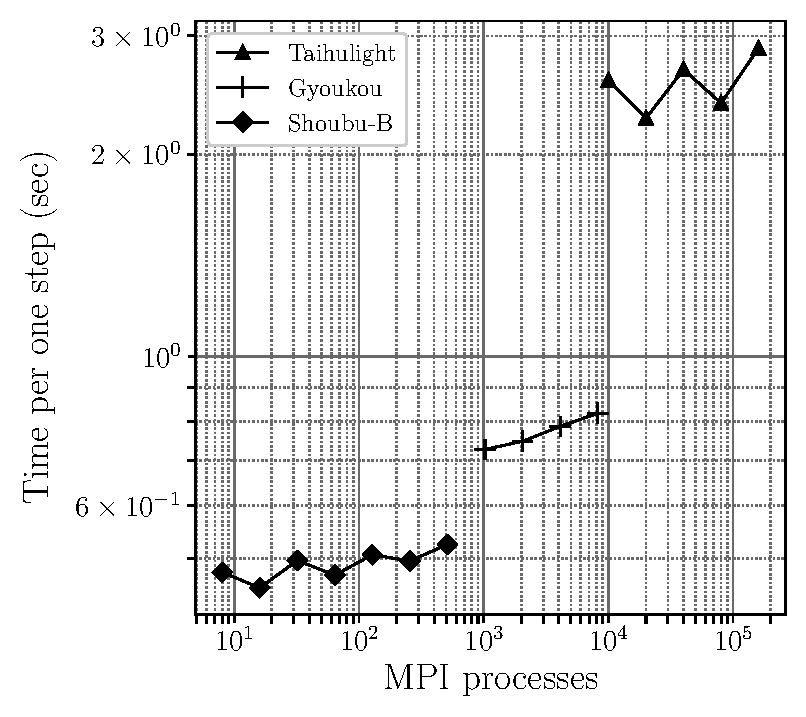
\includegraphics[width=3in]{weak_scaling2}
\caption{Time per timestep for weak-scaling test. The number of
  particles per process is 1M. Here, $n_c$ is the maximum nuber of
  particles to share the interaction list.}
\label{fig:weak}
\end{figure}

\begin{figure}
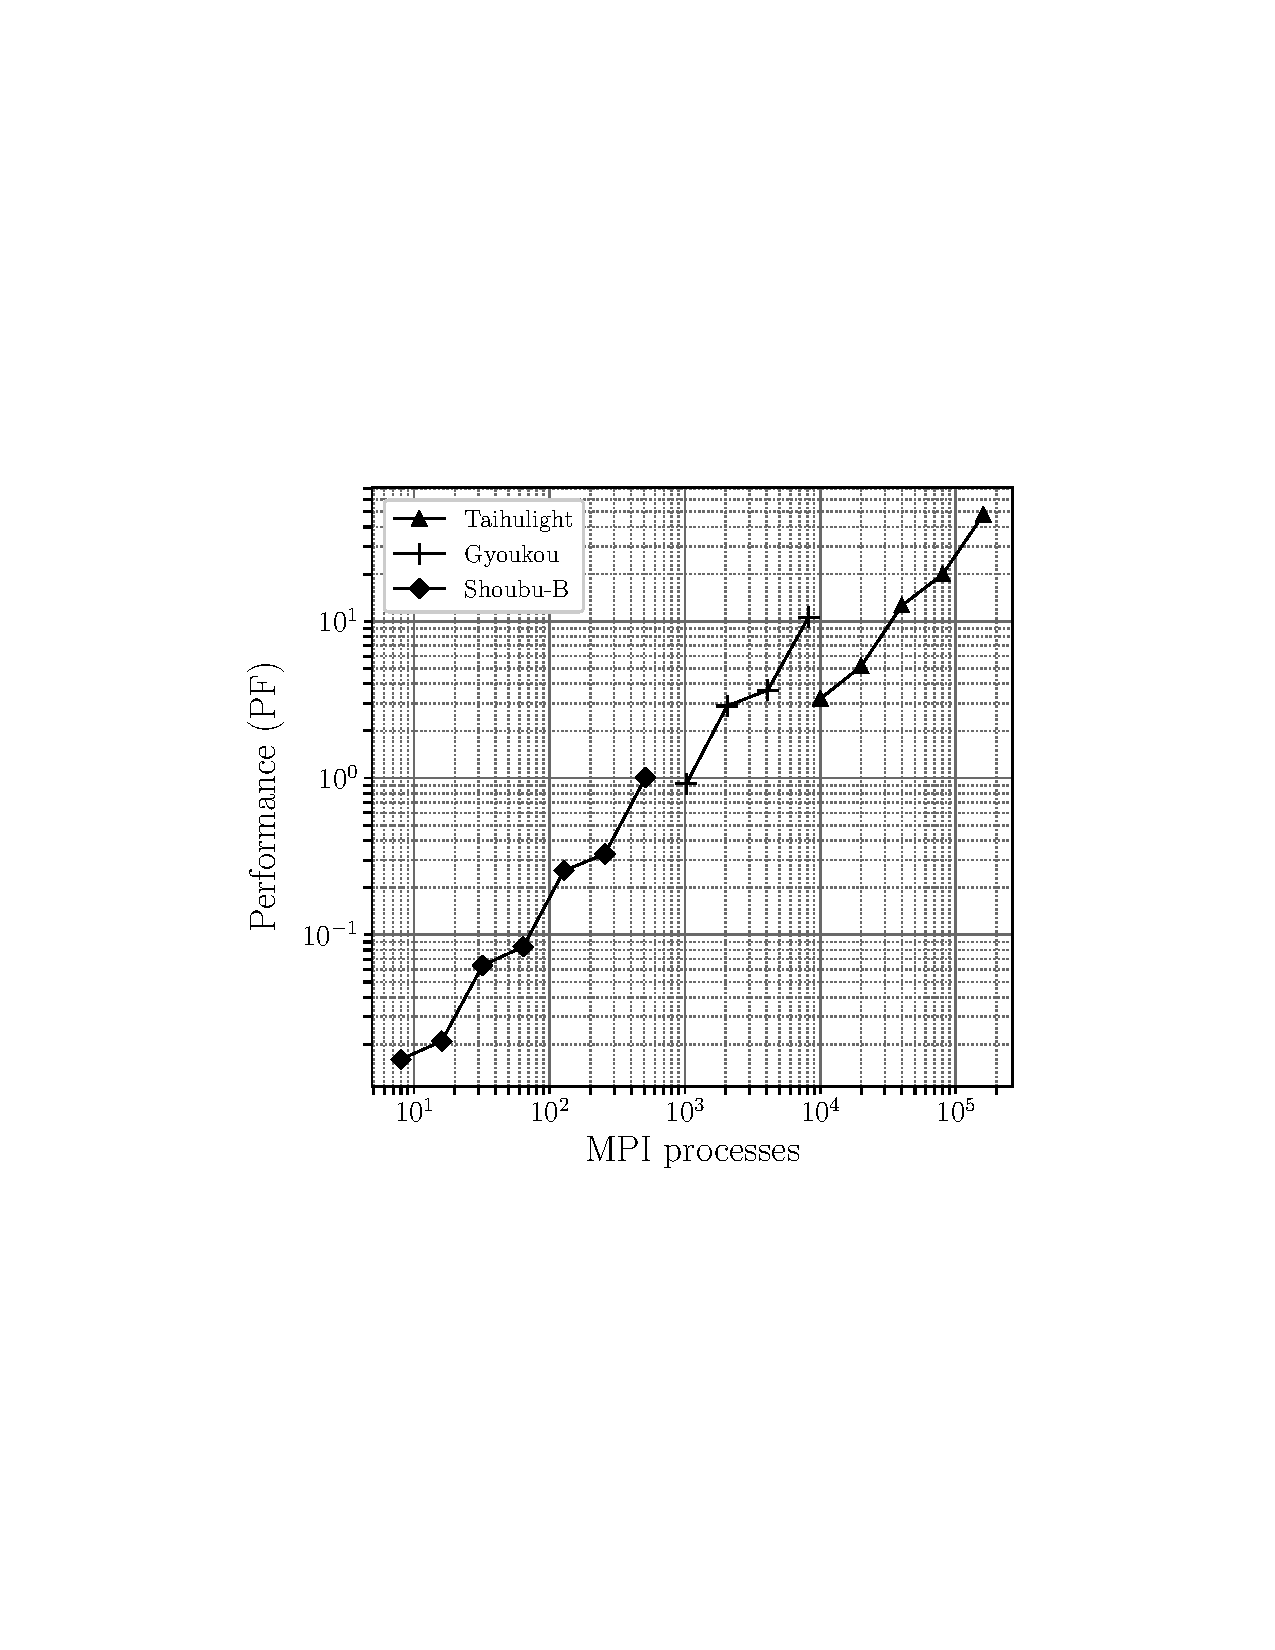
\includegraphics[width=3in]{weak_scaling_speed}
\caption{Performance in petaflops for weak-scaling test. The number of
  particles per process is 1M. Here, $n_c$ is the maximum nuber of
  particles to share the interaction list.}
\label{fig:weakpf}
\end{figure}

\begin{figure}
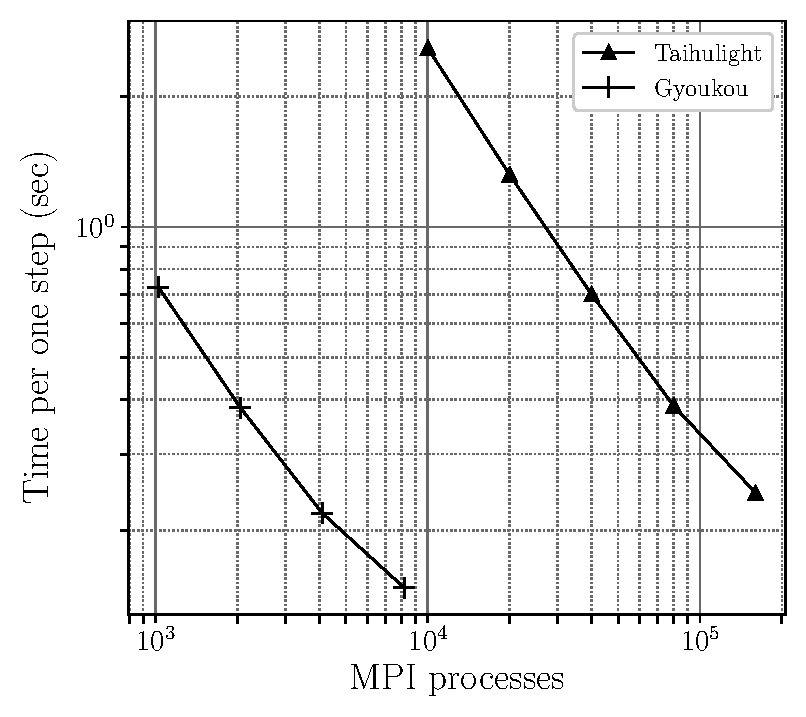
\includegraphics[width=3in]{strong_scaling}
%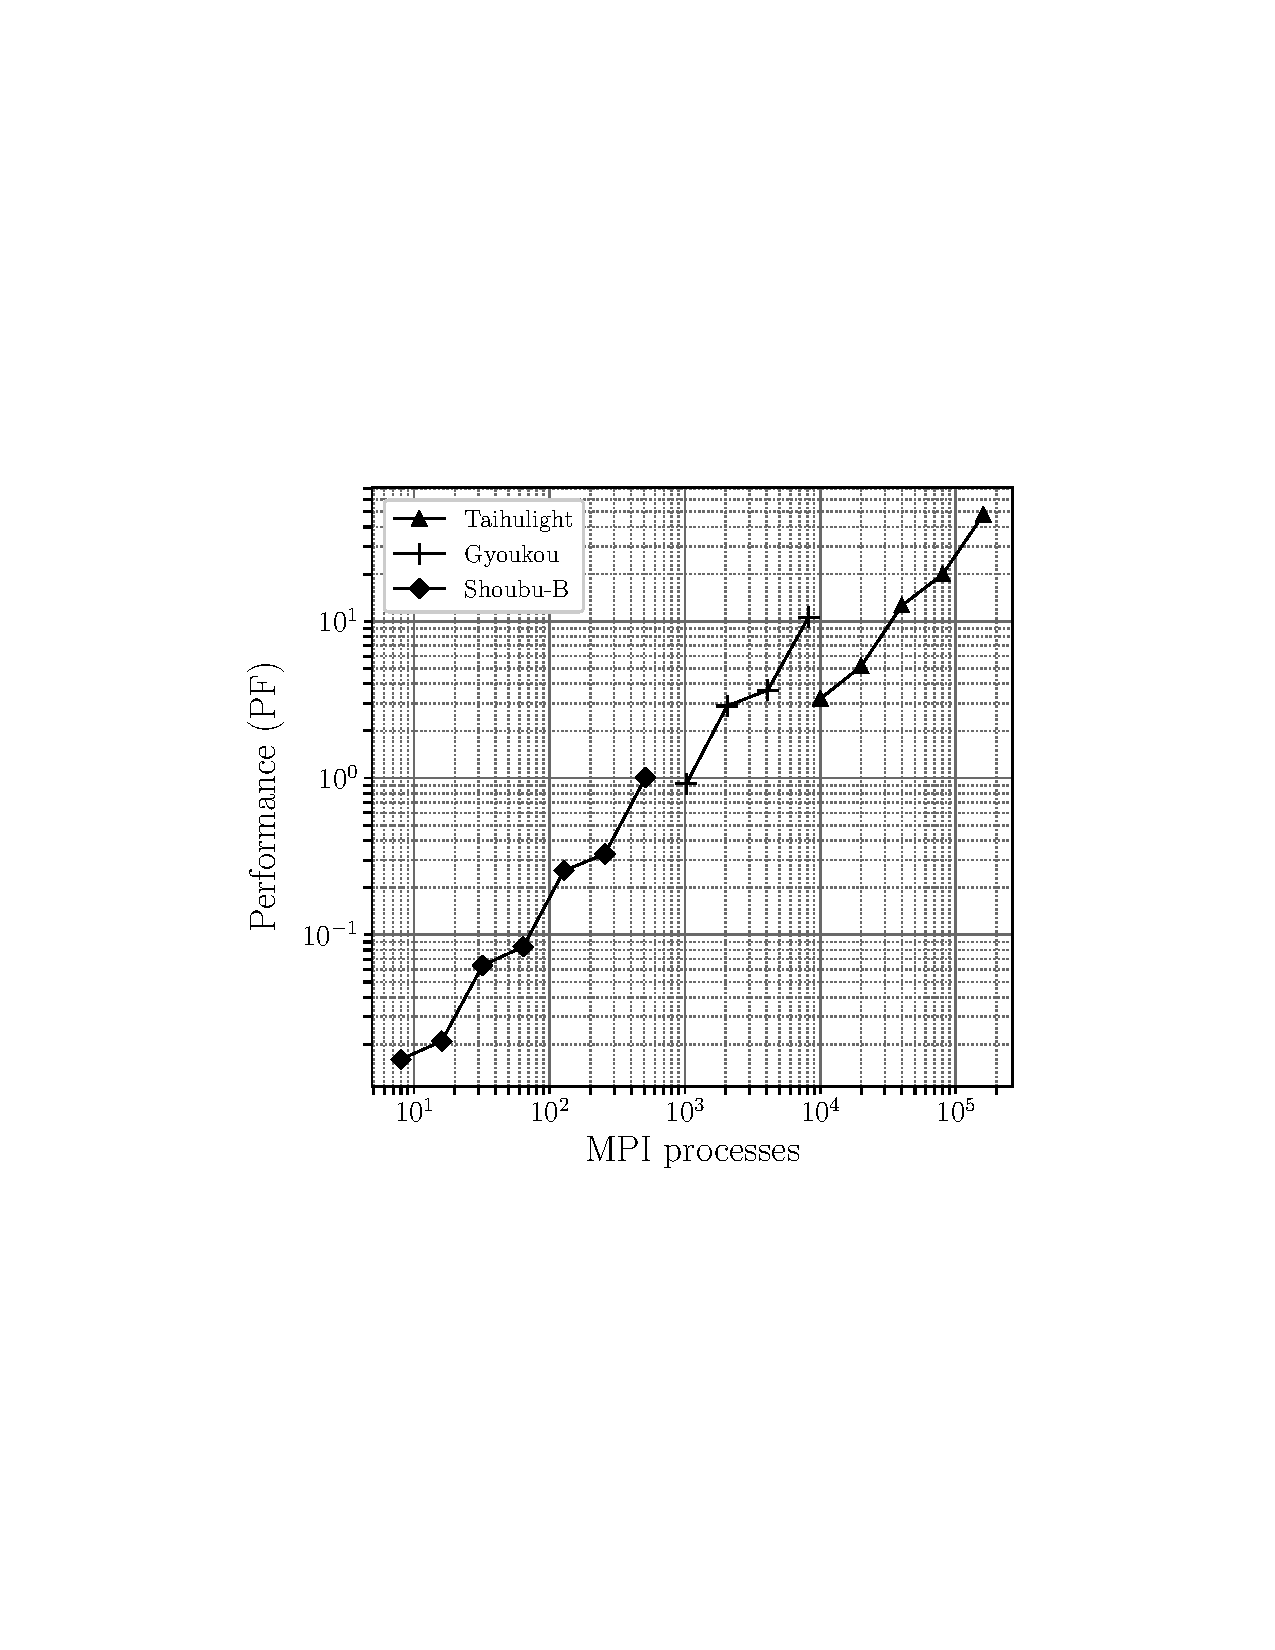
\includegraphics[width=3in]{weak_scaling_speed}
\caption{Time per timestep for strong-scaling test. The total number of
  particles is 32768M.}
\label{fig:strong}
\end{figure}


Figures \ref{fig:weak} and \ref{fig:weakpf}  shows the time per one timestep, for both the strong and
weak scaling measurements. We can see that the weak scaling
performance is quite good. Since our main scientific target is runs
with very large number of particles which has been impossible,
weak-scaling performance is our main interest.

\begin{table}
  \caption{Breakdown of calculation time for weak-scaling runs}
  \label{tab:timeweak}
  \begin{tabular}{cccc}
    \toprule
    \# processes & interaction & comm. & others\\
    \midrule 
    32768 & 0.315587 & 0.0492804&   0.2969116\\
    65536 &    0.41148 &  0.04080394&  0.28833606 \\
131072  & 0.328144 & 0.0588156  & 0.3251454\\
  \bottomrule
\end{tabular}
\end{table}

\begin{table}
  \caption{Breakdown of calculation time for strong-scaling runs}
  \label{tab:timestrong}
  \begin{tabular}{cccc}
    \toprule
    \# processes & interaction & comm. & others\\
    \midrule 
32768   &  0.562725 & 0.0316104 & 0.2756046\\
65536   &  0.332757 & 0.0730505 & 0.1796985\\
131072  &  0.220525 & 0.0535717 & 0.1822023\\
  \bottomrule
\end{tabular}
\end{table}

Tables  \ref{tab:timeweak} and  \ref{tab:timestrong}
  show the breakdown of the calculation time per one
timestep, again for both the weak and strong scaling runs. As
expected, in the case of strong-scaling runs, the calculation  tme for
communication does not decrease. As already stated, our main interest is to
use very large number of particles. Therefore, for actual scientific
runs, the communication time  would not become the limiting
factor.

The performance of run for 128G particles on 32768 nodes is 10.1 PF, or
11.1\% of the theoretical peak performance of the Sunway TaihuLight
system.


We can see that though the weak and strong scaling results are good,
the absolute performance, in terms of the efficiency, is not very high
yet. The efficiency of the interaction kernel is pretty high. We have
threee different interaction kernels, one for particle-particle
interaction, another for particle-tree node interaction, and the last
one for particle-satellite interaction. The inner kernel for these
interactions are written almost completely in assembly language,
except for part of back reaction to satellite particles. Calculation
cost of satellites is only a small fraction of the total cost, since
the number of satellites is limited to 64 in our current calculation.

When we measure the number of cycles per iteration for these three
loops, on average they are  54, 28.7, and 100 for particle-particle,
particle-cell and particle-satellite interactions, respectively, for
SIMD evaluation of interactions to four particles.  The
number of floating-point operations are 47, 31, and 62. Thus, the
efficiencies of the interaction kernels are 43.5\%, 55.7\%, and 32.0\%,
respectively. The theoretical limit for the efficiency of these
kernels is around 60\%, since not all opeations can be done in the
form of FMA.  Thus, interaction kernels are quite well optimized.

On the other hand, actual efficiency achieved  in the interaction calculation
is half of those of kernels.


The primary cause of the loss of the efficiency is most likely the
load imbalance between CPEs. In our current implementation, MPE 
assigns equal number of interaction lists to each CPEs. Since the
there is some fluctuation in the length of the interaction list, the
actual calculation time is not well balanced in our current
implementation.

The length of the interaction list is not the only reason for the
performance fluctuations of CPEs. They can issue DMA request
individually, and the DMA controller processes the requests
sequentially (maybe with some overlap). Thus, even if all CPEs
initiate DMA simultaneously, they receive the result sequentially,
resulting in a rather large difference in the time to finish DMA. This
difference can grow furter, resulting in rather large difference in 
calculation times of CPEs. 

 In terms of the number of
particles integrated per second, we have achieved $2\times
10^{11}$ particles per second, which is about 5 times faster than previous works on
K computer\cite{Ishiyamaetal2012} or ORNL Titan
\cite{Bedorfetal2014}.
\section{Implications}

%  implications for future systems and applications (1 p max)

In this paper, we described the implementation and performance of
a highly efficient simulation code for self-gravitating planetary
rings on the Sunway TaihuLight system.

The measured performance is 10.1 PF, or 11.1\% of the theoretical peak,
for simulation of 128G particles on 32,768 nodes.

Taking into account the unique architecture of the SW26010 processor
used in the TaihuLight system, we regard the achieved performance is
quite high. 

Compared to other multi-core processors for modern  HPC systems such
as Fujitsu SPARC64 VIIIfx and IXfx or Intel Xeon Phi processors,
SW26010 has several unique features which allow very high peak
performance but at the same time make it much harder to achieve high
efficiency on real applications. These are

\begin{itemize}

  \item Heterogeneous architecture with rather extreme ratio of 1:64
    for the number of MPE and CPE
  \item The lack of cache hierarchy for CPE and very limited LDM with
    only 64KB
  \item Very limited main memory bandwidth of effectively 20GB/s for
    one CG, which corresponds to B/F (bytes per flops) ratio of only
    0.03. This is about 1/10 of the numbers of Fujitsu or Intel HPC processors.
    
\end{itemize}  

On the other hand, SW26010 comes with very well-thought features which
allows the programmers to optimize the performance of code on
CPE. These features include
\begin{itemize}

\item Low-latency DMA controller which can be initiated by any CPE.
\item Low-latency, high-bandwidth communication between CPEs
  
\end{itemize}  

These two features allow very efficient use of the main memory
bandwidth. The two-dimensional structure of the network within CG seem
to be optimized for highly efficient implementation of matrix-matrix
multiplications, but it is actually quite useful for other real
applications, whenever fast inter-core communication is necessary.

It is certainly true that the need to use DMAs for data transfer
between CPE and main memory complicates the use of CPE. However, it is
also true that it makes quite optimized access to main memory
possible, since the application programmer can (or have to) control
all main memory accesses. In the case of our code, in several places
we have ``vectorizable'' loop, which perform the same operation on all
particles in the system. The number of operations per particle is
relatively small, of the order of ten, and the data size of one
particle is 32 bytes. In the case of manycore architecture with
hierarchical cache memory, to achieve high efficiency on simple vector
operations like 

{\tt a[i] =   b[i]+c[i]}

is actually quite complicated. In modern processors, load address
would be predicted and hardware prefetch is generated. The hardware
prefetch would probably work for a very simple loop like the above
example, but would fail if many vectors are loaded. Then the
programmer need to experiment with software prefetch, to find the way
to get best performance. 

In the case of SW26010, currently it is rather tedious and error-prone
to write the equivalent operation using the combination of Athread and
DMA, and sometimes inner kernel in assembly language, but once you do
so, you can get a performance close to performance estimate from
simple model based on DMA communication performance. 

The existence of low-latency (less than 10 clock cycles) communication
path between is quite important for using CPEs for fine-grain
parallelism such as loop-level parallelization. Such low-latency
communication is difficult to implement on shared memory processors
with hierarchical cache. Fujitsu processors are exceptional in this
aspect, in supporting very fast hardware barrier instruction, but this
barrier covers only the processors that physically share L2D cache.

In the current implementation, we have not yet used CPEs for complex
operations such as  tree traversal. However, to
implement these operations using DMA is possible, and then we can
further reduce the amount of work currently done on MPE.

One  problem with the current software/hardware system is that writing
high-performance kernel for CPE currently means writing the inner
kernel in assembly language. This is purely the software limitation,
and probably not so difficult to fix.

In conclusion, we have implemented parallel particle simulation code
on Sunway SW26010 processor, and found that its rather extreme
architecture is actually quite suitable for achieving high performance
for carefully designed algorithm. Even though the B/F number is only
0.03 and the network bandwidth is similarly low, the efficiency we
have achieved is not too different from that on K computer, with 15
times more memory and network bandwidth. We feel that architecture
evolution in this direction will help the HPC community to continue
improving the performance.



\bibliographystyle{ACM-Reference-Format}
%\bibliography{sigproc} 


\bibliography{../../bibtex/allrefs}

  
\end{document}
